\section{Fault impact analysis}
In Section~\ref{sec:empirical}, we showed that a transient fault may have a significant impact on the convergence of an execution. In this section, an analysis is proposed to evaluate this impact. We first describe the error propagation through the different steps of the algorithm in ~\ref{sec:propagation}, to observe which variables are altered, and then we analytically quantify the error in~\ref{sec:quantify}, in order to intent to predict the convergence behavior in~\ref{sec:prediction}.


\subsection{Error propagation}\label{sec:propagation}
At the fault iteration $i=f$, some variables become corrupted as illustrated in Figure \ref{fig:error_propagation}. At first, only one value in the vector $w = A \cdot v_f$ is erroneous, but this error gets spread out in the orthonormalization process (modified Gram-Schmidt), generating a wrong new arnoldi vector $v_{f+1}$ as well as a wrong last column in the Hessenberg matrix $H_{f+1}$, resulting in a different Krylov space and potentially leading to an incorrect solution. Moreover, the erroneous Arnoldi basis ($V_{f+1}$) and Hessenberg matrix ($H_{f+1}$) are used in the next iterations, which may increasing the deviation from the correct execution even further. 
\begin{figure}[h]
\centering
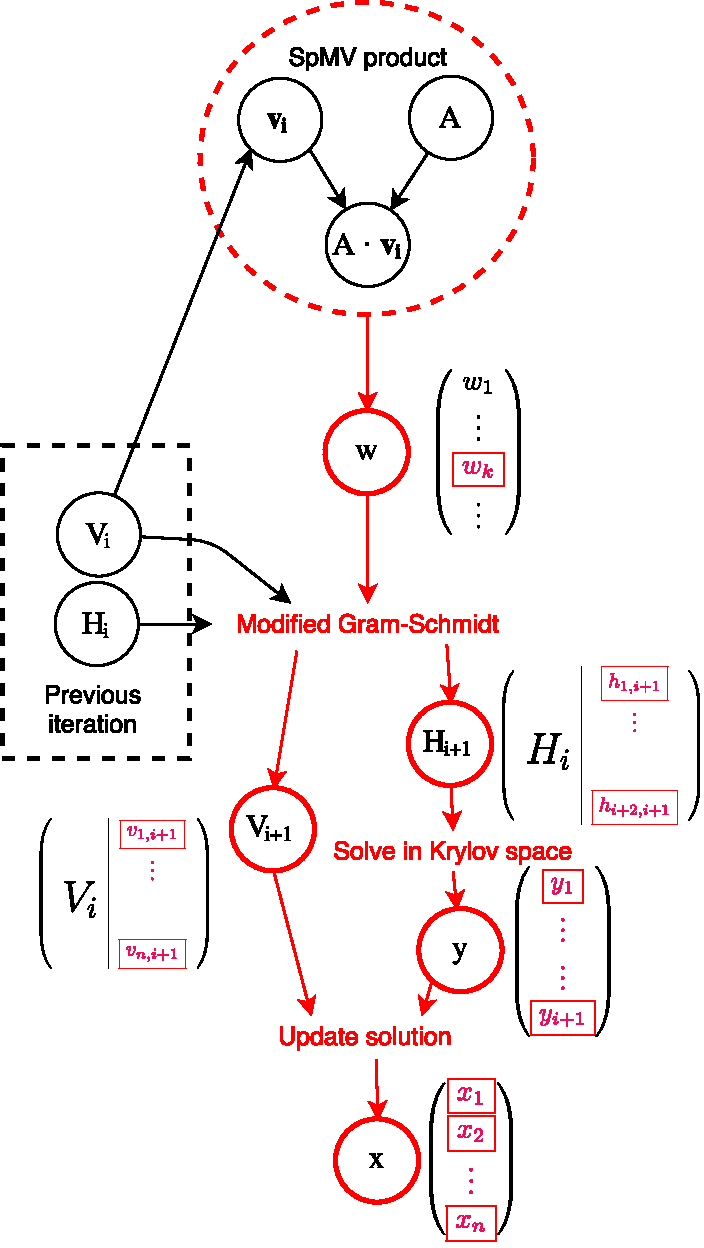
\includegraphics[scale=0.5]{figures/error_propagation.pdf}
\caption{Error (red) propagation at the fault iteration.}\label{fig:error_propagation}
\end{figure}

\subsection{Error quantification}\label{sec:quantify}
Because the sequence of least-square problems solved along the iteration are nested; that is at iteration $i$ 
the leading part of $H_{i+1}$ is $H_i$ as well as for the right-hand sides; we know that independently of the possible occurrence of a fault during the execution, GMRES always reduces the computed residual norm down to the machine accuracy, as long as it is given enough iterations to do so. However, a fault may introduce a large residual deviation between the computed residual and the true residual (i.e., $\|\widetilde{r}_{\ell} - \widetilde{r}_{\ell}\textprime \|$ becomes large), which may prevent the latter one from reaching the target accuracy. Since $ \|\widetilde{r}_{\ell}\| \geq \|\widetilde{r}_{\ell} - \widetilde{r}_{\ell}\textprime \| - \| \widetilde{r}_{\ell}\textprime \|$ and $\|\widetilde{r}_\ell\textprime \| \rightarrow 0$, we obtain that $\|\widetilde{r}_{\ell}\| \rightarrow \|\widetilde{r}_{\ell} - \widetilde{r}_\ell\textprime \|$, so if the error remains greater than the target accuracy $\varepsilon$, the execution will not converge. The error measured at iteration $\ell$ is called the residual gap at iteration $\ell$, denoted $\delta(\ell)$.
We illustrate in figures \ref{fig:gre_216a_conv_hist_delta} and \ref{fig:pores_2_conv_hist_delta} the effect of a soft-error on the norm of the residuals and the residual gap.
The red curve, the true residual $\|\widetilde{r}_{\ell}\|$, and the light blue curve, the residual gap $\delta(\ell)$, get closer and closer as the green curve, the computed residual $\|\widetilde{r}\textprime_{\ell}\|$, is reduced down to the machine accuracy.
The dashed blue line shows the non-faulty execution residuals, to illustrate the delay induced by the error in the convergence.
The residual gap provides a good quantification of the fault impact, however it does not explain nor quantifies how much the convergence is delayed (when the convergence occurs).




\begin{figure}[h]
	\centering
	\begin{subfigure}[t]{0.45\linewidth}
		\centering
		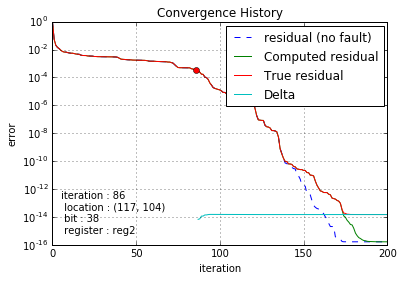
\includegraphics[width=1.1\linewidth]{figures/gre_216a/convergence_history_delta.png}
		\caption{GMRES on gre_216a}\label{fig:gre_216a_conv_hist_delta}		
	\end{subfigure}
	\quad
	\begin{subfigure}[t]{0.45\linewidth}
		\centering
		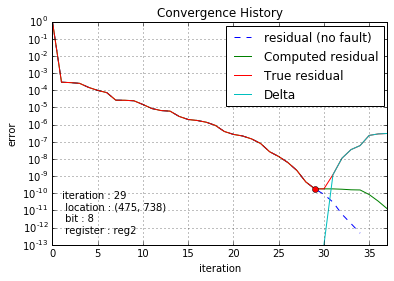
\includegraphics[width=1.1\linewidth]{figures/pores_2/convergence_history_delta.png}
		\caption{preconditioned-GMRES on pores_2, }\label{fig:pores_2_conv_hist_delta}
	\end{subfigure}
    \caption{Two convergence histories disrupted by a fault. The light blue line represents the residual gap evolution in the faulty executions:GMRES on gre_216a in \ref{fig:gre_216a_conv_hist_delta} and precondition-GMRES  on pores_2 in \ref{fig:pores_2_conv_hist_delta}.}
\end{figure}



%TODO y-axis error

In~\cite{sisz:03}, the authors provide a general framework for the understanding of inexact Krylov subspaces, generated by inexact matrix vector products that arise naturally in many scientific applications. In particular, they analyze the residual norm deviation assuming that a perturbation $E_i$ is applied to the SpMV product at each
iteration $i$. 
\begin{equation}\label{inexact_krylov}
 \widetilde{r}_\ell = \widetilde{r}_\ell\textprime + \widetilde{y_\ell} \cdot \sum_{i=1}^{\ell}{E_i \cdot v_i}
 \end{equation}

We can use this analysis in a somehow simpler situation where a transient fault is considered as a perturbation $E_f$ that only occurs once at the $f^{th}$ iteration, specializing the results in ~\cite{sisz:03} to be applicable in our model.
\begin{equation}\label{inexact_krylov_adapted}
\| \widetilde{r}_\ell - \widetilde{r}_\ell\textprime \| =  \| \widetilde{y_\ell} \cdot E_f \cdot v_f \|
 \end{equation}

This enables us to get the following equation that links the residual gap to the $\widetilde{y}_{\ell, f}$ evolution and the error introduced by the fault $\|E_f \cdot v_f\| = \|A \cdot {v}_{f} - \widetilde{A} \cdot v_{f}\| = \|{w}_{f+1} - \widetilde{w}_{f+1}\|$ :
\begin{equation}\label{eqn:delta}
\delta(\ell) = \|\widetilde{r}_{\ell} - \widetilde{r}_{\ell}\textprime \| = |\widetilde{y}_{{\ell}, f}|\cdot \|{w}_{f+1} - \widetilde{w}_{f+1}\|
\end{equation}
where  $w_{f+1}$ is the $f+1^{th}$ Arnoldi vector before orthonormalization and $\widetilde{y}_{\ell, f}$ is the $f^{th}$ component of the $\ell^{th}$ least square problem solution $\widetilde{y}_\ell=\argmin_{\mathbf{y_{}}}\|\beta e_1 - H_{\ell} \mathbf{y_{}}\|$.

\subsection{Prediction of the fault impact}\label{sec:prediction}
From Section~\ref{sec:empirical}, we observed that faults may either have a critical impact when preventing the execution from converging, little impact when delaying the convergence, or no impact at all. Ideally, by using the symptoms brought by a fault we should be able to predict its impact.


Theorem~\ref{theorem} below proposes a possible suited criterion in the form of a threshold on the error $\|{w}_{f+1} - \widetilde{w}_{f+1}\|$ to ensure that a fault is not critical.
It is based on Equation~\eqref{eqn:delta}, itself relying on the remark that a faulty matrix-vector product caused by a bit-flip can be interpreted as an inexact matrix-vector product in inexact~\cite{sisz:03} or
relaxed~\cite{DBLP:journals/siamsc/GiraudGL07} GMRES.
\begin{theorem}\label{theorem}
Let $0 < c < 1$ and let a GMRES execution using $(1-c) \varepsilon$ as the target accuracy, terminating in $\ell$ iterations and disrupted by a fault at iteration $f < \ell$. In exact arithmetic, if $\|{w}_{f+1} - \widetilde{w}_{f+1}\| < \tau_c = (c \cdot \varepsilon) / |\widetilde{y}_{\ell, f}|$ then the execution converges to the target accuracy $\varepsilon$.
\end{theorem}
\begin{proof}
The purpose of the $c$ parameter is to bound the true residual norm as a convex combination of the residual deviation norm and the computed residual norm.
Since the GMRES execution terminates in $\ell$ iterations for the target accuracy $(1 - c) \varepsilon$ $$\|\widetilde{r}\textprime_{\ell}\| \leq (1 - c) \varepsilon$$
Then, using Equation \eqref{eqn:delta} derived from \cite{DBLP:journals/siamsc/GiraudGL07} and the criterion $\|{w}_{f+1} - \widetilde{w}_{f+1}\| < \frac{c \cdot \varepsilon}{|\widetilde{y}_{\ell, f}|}$ :

\begin{equation}
%
\begin{split}
    \|\widetilde{r}_\ell\| & \leq \|\widetilde{r}_\ell - \widetilde{r}\textprime_\ell \| + \|\widetilde{r}\textprime_\ell\| \\
    &\leq \|y_{\ell, f} (w_{f+1} - \widetilde{w}_{f+1}) \| + \|\widetilde{r}\textprime_\ell\| \\
    &\leq |y_{\ell, f}| \cdot \|{w}_{f+1} - \widetilde{w}_{f+1}\| + \|\widetilde{r}\textprime_\ell\| \\
     &\leq c \cdot \varepsilon + (1 - c) \cdot \varepsilon = \varepsilon\\
%
\end{split}
\end{equation}
The GMRES execution has converged with the target accuracy $\varepsilon$.
\end{proof}
Let $0 < c < 1$, and a faulty execution whose target accuracy is set to $(1 - c) \cdot \varepsilon$. Using Theorem~\ref{theorem}, we can predict if the fault will not disrupt the convergence to $\varepsilon$ by computing the following expression:
\begin{equation}
	\text{error} = \|{w}_{f+1} - \widetilde{w}_{f+1}\| < \tau_c = (c \cdot \varepsilon) / |\widetilde{y}_{\ell, f}|
\end{equation}\label{scheme_oracle}
If the threshold is greater than the error, the execution must converge to the target accuracy $\varepsilon$ according to Theorem \ref{theorem}. Note that the reverse is not necessarily true so if the error is greater than the threshold, the execution may or may not converge to the target accuracy. 

%Table \ref{table:theoretical_outcomes} gathers the 4 possible outcomes produced by this detection scheme. If the execution converges, the fault is said to have no impact, whereas a fault preventing the execution from converging is said to be critical. 

% \begin{table}[h]
% \centering
% \caption{Colors and name used for each test outcome.}
% \label{table:theoretical_outcomes}
% \begin{tabular}{l|ll|}
% 	& Convergence & No convergence\\
%     \hline
%    Detection & \color[RGB]{30, 30, 30}{\textbf{No impact fault detected}} & \color[RGB]{85, 147, 47}{\textbf{Critical fault detected}} \\
 
%    No detection & \color[RGB]{90, 90, 90}{\textbf{No impact fault ignored}} & \color{red}{\textbf{Critical fault ignored}} \\
%     \hline
% \end{tabular}
% \end{table}

% Figure \ref{fig:conv_hist_detection_correct} plots 2 convergence histories for each algorithm. In figures \ref{fig:gre_216a_conv_hist_theoretical_detection_0} and 
% \ref{fig:pores_2_conv_hist_theoretical_detection_0}, no fault is detected as the error is smaller than the threshold, and the executions converges, producing a \emph{No impact fault ignored} from Table~\ref{table:theoretical_outcomes}. In figures \ref{fig:gre_216a_conv_hist_theoretical_detection_1} and 
% \ref{fig:pores_2_conv_hist_theoretical_detection_1}, a critical fault is detected as the error is greater than the threshold $\tau_{0.5}$ at the fault iteration and the executions does not converge, producing a \emph{Critical fault detected} from Table~\ref{table:theoretical_outcomes}. In both cases, the fault is properly detected.






% \begin{figure}[h]
% 	\centering
    
% \begin{minipage}[b]{0.45\linewidth}
% \centering
% \textbf{full-GMRES} executions on \textbf{gre_216a} 
% \end{minipage}
% \quad
% \begin{minipage}{0.45\linewidth}
% \centering
% \textbf{preconditioned-GMRES} on \textbf{pores_2}
% \end{minipage}\\


%     \begin{minipage}[b]{0.48\linewidth}
	
% 	\begin{subfigure}[t]{\linewidth}
% 		\centering
% 		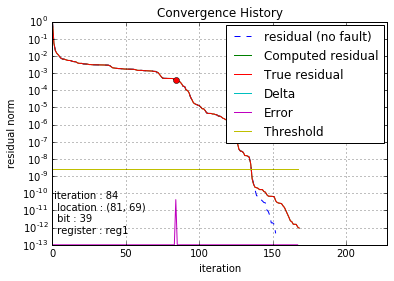
\includegraphics[width=\linewidth]{figures/gre_216a/convergence_history_theoretical_detection_1_1.png}
% 		\caption{No impact fault ignored}\label{fig:gre_216a_conv_hist_theoretical_detection_0}
% 	\end{subfigure}
%     \quad
%     \begin{subfigure}[t]{\linewidth}
% 		\centering
% 		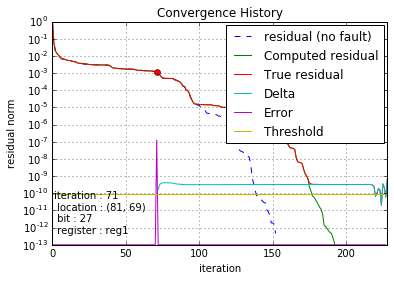
\includegraphics[width=\linewidth]{figures/gre_216a/convergence_history_theoretical_detection_0_1.png}
% 		\caption{Critical fault detected}\label{fig:gre_216a_conv_hist_theoretical_detection_1}
% 	\end{subfigure}
%     \end{minipage}
%     \quad
%     \begin{minipage}[b]{0.48\linewidth}
    	
% 	\begin{subfigure}[t]{\linewidth}
% 		\centering
% 		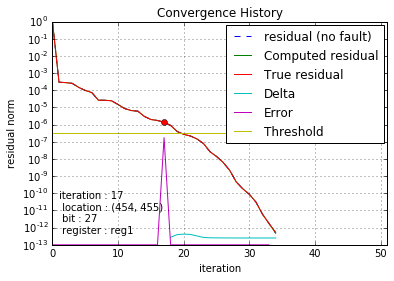
\includegraphics[width=\linewidth]{figures/pores_2/convergence_history_theoretical_detection_1_1.png}
% 		\caption{No impact fault ignored}\label{fig:pores_2_conv_hist_theoretical_detection_0}
% 	\end{subfigure}
%     \quad
%     \begin{subfigure}[t]{\linewidth}
% 		\centering
% 		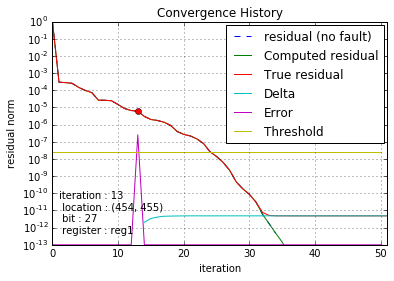
\includegraphics[width=\linewidth]{figures/pores_2/convergence_history_theoretical_detection_0_1.png}
% 		\caption{Critical fault detected}\label{fig:pores_2_conv_hist_theoretical_detection_1}
% 	\end{subfigure}

    
% 	\end{minipage}
% \caption{Convergence histories of 2 full-GMRES executions on HB/gre_216a and 2 preconditioned-GMRES executions on HB/pored_2, disrupted by transient faults that are properly detected. The error and the threshold are plotted. In figures~\ref{fig:gre_216a_conv_hist_theoretical_detection_0} and~\ref{fig:pores_2_conv_hist_theoretical_detection_0}, the error at each iteration remains below the threshold, so no fault is detected and the execution converges, producing a \emph{No impact fault ignored} from Table \ref{colors}. In figures~\ref{fig:gre_216a_conv_hist_theoretical_detection_1} and~\ref{fig:pores_2_conv_hist_theoretical_detection_1}, the error becomes higher than the threshold at the fault iteration, so the fault is detected and the execution does not converge, producing a \emph{Critical fault detected} from Table \ref{table:theoretical_outcomes}. }\label{fig:conv_hist_detection_correct}
% \end{figure}





 \subsection{Numerical experiment}
 Figure~\ref{fig:detection} displays the 
 
 

\begin{figure}[h]
	\centering
    
\begin{minipage}[b]{0.45\linewidth}
\centering
\textbf{GMRES} executions on \textbf{gre_216a} 
\end{minipage}
\quad
\begin{minipage}{0.45\linewidth}
\centering
\textbf{preconditioned-GMRES} on \textbf{pores_2}
\end{minipage}\\


    \begin{minipage}[b]{0.48\linewidth}
	\begin{subfigure}[t]{\linewidth}
		\centering
		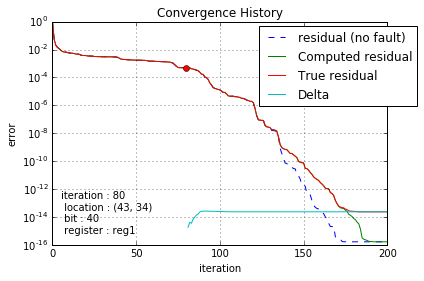
\includegraphics[width=\linewidth]{figures/gre_216a/convergence_history_location_0.png}
		\caption{}\label{fig:gre_216a_conv_hist_location_0}		
	\end{subfigure}
	\quad
	\begin{subfigure}[t]{\linewidth}
		\centering
		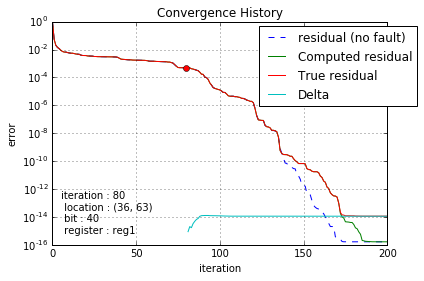
\includegraphics[width=\linewidth]{figures/gre_216a/convergence_history_location_1.png}
		\caption{}\label{fig:gre_216a_conv_hist_location_1}
	\end{subfigure}
    \quad
    \begin{subfigure}[t]{\linewidth}
		\centering
		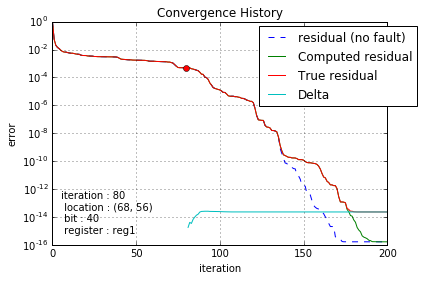
\includegraphics[width=\linewidth]{figures/gre_216a/convergence_history_location_2.png}
		\caption{}\label{fig:gre_216a_conv_hist_location_2}
	\end{subfigure}
    \end{minipage}
    \quad
    \begin{minipage}[b]{0.48\linewidth}
    	\begin{subfigure}[t]{\linewidth}
		\centering
		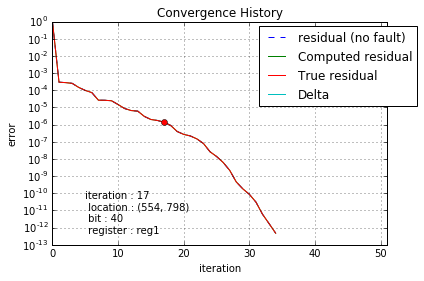
\includegraphics[width=\linewidth]{figures/pores_2/convergence_history_location_0.png}
		\caption{}\label{fig:pores_2_conv_hist_location_0}		
	\end{subfigure}
	\quad
	\begin{subfigure}[t]{\linewidth}
		\centering
		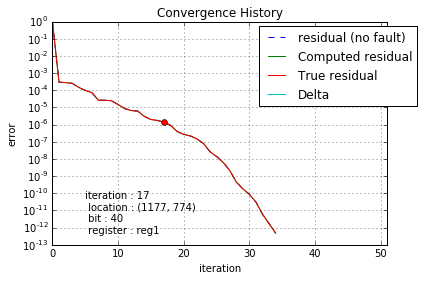
\includegraphics[width=\linewidth]{figures/pores_2/convergence_history_location_1.png}
		\caption{}\label{fig:pores_2_conv_hist_location_1}
	\end{subfigure}
    \quad
    \begin{subfigure}[t]{\linewidth}
		\centering
		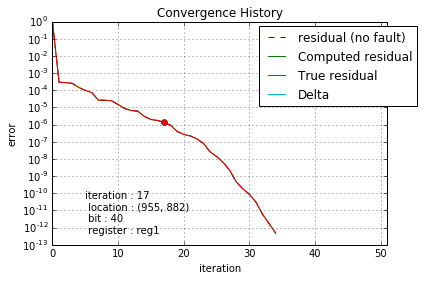
\includegraphics[width=\linewidth]{figures/pores_2/convergence_history_location_2.png}
		\caption{}\label{fig:pores_2_conv_hist_location_2}
	\end{subfigure}

    
	\end{minipage}
	\caption{Convergence history of 3 GMRES executions on gre_216a and 3 preconditioned-GMRES executions on pores_2, disrupted by a transient fault. In all the executions, the faults (occurring in random locations) seem to have the same impact.}\label{fig:prediction}
\end{figure}



% Figure~\ref{fig:test_result_oracle} displays the fault detection scheme results (in percentage of executions) for several values of c.
% First, no critical faults are ignored, which is a direct consequence of Theorem \ref{theorem}: If a fault Second, for low values of $c$, an important part (between 20\% and 35\%) of executions disrupted by a negligible fault detect it anyway (dark gray) as the detection scheme is more sensitive, but it becomes more and more capable of ignoring those when $c$ increases. The rest of the faulty executions (green and light gray) are correctly handled.

% For more details, the $c=0.5$ cases are plotted in Figure~\ref{fig:test_result_c05}. In each case, all the critical fault are correctly detectedlarge majority of the faulty executions correctly detects the faults. The rare cases of unneeded detection (dark gray) occur at the limit of the convergence and non convergence domain (light gray and green respectively).





% \begin{figure}[h]
% 	\centering
    
% \begin{minipage}[b]{0.45\linewidth}
% \centering
% \textbf{full-GMRES} executions on \textbf{gre_216a} 
% \end{minipage}
% \quad
% \begin{minipage}{0.45\linewidth}
% \centering
% \textbf{preconditioned-GMRES} on \textbf{pores_2}
% \end{minipage}\\


%     \begin{minipage}[b]{0.48\linewidth}
	
% 	\begin{subfigure}[t]{\linewidth}
% 		\centering
% 		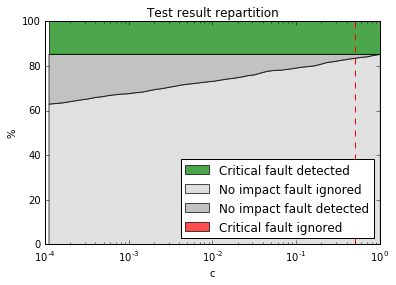
\includegraphics[width=1.1\linewidth]{figures/gre_216a/test_result_oracle_0.png}
% 		\caption{$\varepsilon = 10^{-6}$}\label{fig:gre_216a_test_result_oracle_0}	
% 	\end{subfigure}
%     \quad
%     \begin{subfigure}[t]{\linewidth}
% 		\centering
% 		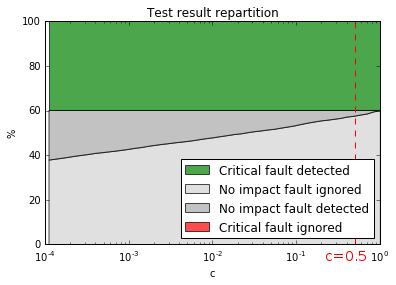
\includegraphics[width=1.1\linewidth]{figures/gre_216a/test_result_oracle_1.png}
% 		\caption{$\varepsilon = 10^{-12}$}\label{fig:gre_216a_test_result_oracle_1}	
% 	\end{subfigure}
%     \end{minipage}
%     \quad
%     \begin{minipage}[b]{0.48\linewidth}
    	
% 	\begin{subfigure}[t]{\linewidth}
% 		\centering
% 		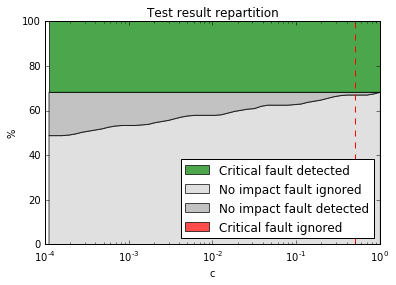
\includegraphics[width=1.1\linewidth]{figures/pores_2/test_result_oracle_0.png}
% 		\caption{$\varepsilon = 10^{-6}$}\label{fig:pores_2_test_result_oracle_0}	
% 	\end{subfigure}
%     \quad
%     \begin{subfigure}[t]{\linewidth}
% 		\centering
% 		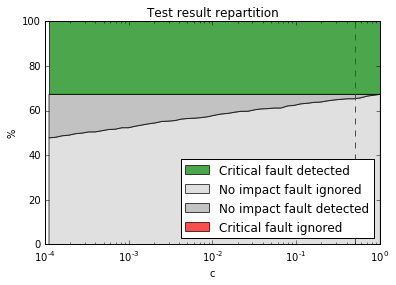
\includegraphics[width=1.1\linewidth]{figures/pores_2/test_result_oracle_1.png}
% 		\caption{$\varepsilon = 10^{-12}$}\label{fig:pores_2_test_result_oracle_1}	
% 	\end{subfigure}

% 	\end{minipage}
% \caption{Diagrams representing the test outcome proportion for several values of c. To compute them, faulty executions covering a large part of the fault parameter space were performed. The case $c = 0.5$ represented by the dashed red line is detailed in Figure~\ref{fig:test_result_oracle_c05}.}\label{fig:test_result_oracle}
% \end{figure}




% \begin{figure}[h]
% 	\centering
    
% \begin{minipage}[b]{0.45\linewidth}
% \centering
% \textbf{full-GMRES} executions on \textbf{gre_216a} 
% \end{minipage}
% \quad
% \begin{minipage}{0.45\linewidth}
% \centering
% \textbf{preconditioned-GMRES} on \textbf{pores_2}
% \end{minipage}\\


%     \begin{minipage}[b]{0.48\linewidth}
	
% 	\begin{subfigure}[t]{\linewidth}
% 		\centering
% 		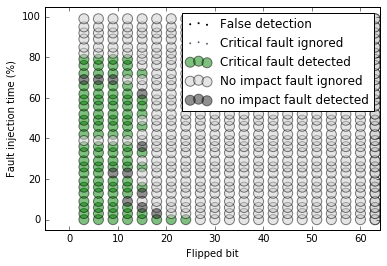
\includegraphics[width=1.1\linewidth]{figures/gre_216a/test_result_c05_oracle_0.png}
% 		\caption{$\varepsilon = 10^{-6}$}\label{fig:gre_216a_test_result_c05_oracle_0}	
% 	\end{subfigure}
%     \quad
%     \begin{subfigure}[t]{\linewidth}
% 		\centering
% 		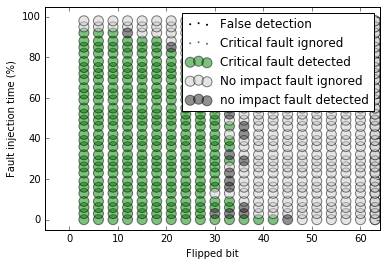
\includegraphics[width=1.1\linewidth]{figures/gre_216a/test_result_c05_oracle_1.png}
% 		\caption{$\varepsilon = 10^{-12}$}\label{fig:gre_216a_test_result_c05_oracle_1}	
% 	\end{subfigure}
%     \end{minipage}
%     \quad
%     \begin{minipage}[b]{0.48\linewidth}
    	
% 	\begin{subfigure}[t]{\linewidth}
% 		\centering
% 		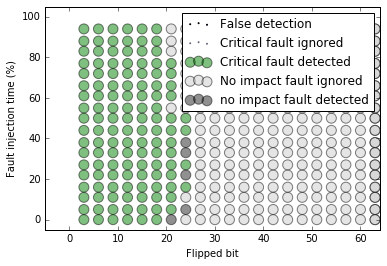
\includegraphics[width=1.1\linewidth]{figures/pores_2/test_result_c05_oracle_0.png}
% 		\caption{$\varepsilon = 10^{-6}$}\label{fig:pores_2_test_result_c05_oracle_0}	
% 	\end{subfigure}
%     \quad
%     \begin{subfigure}[t]{\linewidth}
% 		\centering
% 		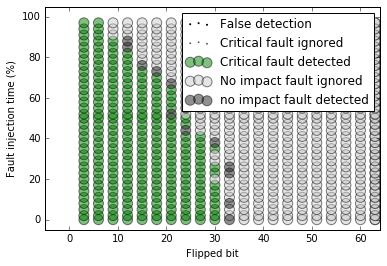
\includegraphics[width=1.1\linewidth]{figures/pores_2/test_result_c05_oracle_1.png}
% 		\caption{$\varepsilon = 10^{-12}$}\label{fig:pores_2_test_result_c05_oracle_1}	
% 	\end{subfigure}

% 	\end{minipage}
% \caption{Diagram detailing the test results for $c = 0.5$. Each dot corresponds to a faulty execution, and its color represents the test outcome from Table \ref{table:theoretical_outcomes}.}
% \label{fig:test_result_oracle_c05}
% \end{figure}


